
%%%%%%%%%%%%%%%%%%%%%%%%%%%%%%%%%%%%%%%%%%%%%%%%%%%%%%%%%%%%%%%%%%%%%%%%%%%%%%%
%
%  EGSnrc GUI maintenance manual
%  Copyright (C) 2015 National Research Council Canada
%
%  This file is part of EGSnrc.
%
%  EGSnrc is free software: you can redistribute it and/or modify it under
%  the terms of the GNU Affero General Public License as published by the
%  Free Software Foundation, either version 3 of the License, or (at your
%  option) any later version.
%
%  EGSnrc is distributed in the hope that it will be useful, but WITHOUT ANY
%  WARRANTY; without even the implied warranty of MERCHANTABILITY or FITNESS
%  FOR A PARTICULAR PURPOSE.  See the GNU Affero General Public License for
%  more details.
%
%  You should have received a copy of the GNU Affero General Public License
%  along with EGSnrc. If not, see <http://www.gnu.org/licenses/>.
%
%%%%%%%%%%%%%%%%%%%%%%%%%%%%%%%%%%%%%%%%%%%%%%%%%%%%%%%%%%%%%%%%%%%%%%%%%%%%%%%
%
%  Authors:         Joanne Treurniet, 1998
%
%  Contributors:
%
%%%%%%%%%%%%%%%%%%%%%%%%%%%%%%%%%%%%%%%%%%%%%%%%%%%%%%%%%%%%%%%%%%%%%%%%%%%%%%%


\documentclass[12pt]{book}

\setlength{\textwidth}{16.51cm}
\setlength{\textheight}{23.5cm}
\setlength{\oddsidemargin}{0.0in}
\setlength{\evensidemargin}{0.0in}
\setlength{\topmargin}{-1.5cm}
\setlength{\parindent}{1.5em}
\setlength{\topsep}{0ex}
\setlength{\itemsep}{0ex}

\newcommand{\Co}{$^{60}$Co}
\newcommand{\parsp}{~\hspace*{1.5em}}
\setlength{\parskip}{0.1in}
\setlength{\baselineskip}{1.0cm}
\newcommand{\head}[1]{\begin{center}\begin{Large}{\bf #1}
                                              \end{Large}\end{center}}
\newcommand{\cen}[1]{\begin{center} #1 \end{center}                   }
\newcommand{\cm}{component module}
\newcommand{\CM}{Component module}
\newcommand{\etal}{{\em et.al.}}
\newcommand{\ie}{{\em i.e.}}
\newcommand{\etc}{{\em etc.}}
\newcommand{\viz}{{\em viz.}}
\newcommand{\eg}{{\em eg.}}

%\renewcommand{\refname}{}

\usepackage{graphicx}

\usepackage{fancyheadings}
\usepackage{html}


\makeindex
\begin{document}

\footrulewidth=0.4pt
\headrulewidth=0.4pt

\lhead[{\sffamily \thepage}]{{\sffamily BEAM GUI Maintenance Guide}}
\rhead[{\sffamily NRCC Report PIRS-0509(A)revB}]{{\sffamily ~\thepage}}
\rfoot[{\sffamily {\rightmark}}]{{\sffamily {\rightmark}}}
\lfoot[{\sffamily {\leftmark}}]{{\small Last edited $Date: 2004/09/09 16:09:23 $
}}
\cfoot{}

\begin{latexonly}
\typeout{***Have turned off overfull and underfull messages****}
\tolerance=10000        %suppress Overfull only
\hbadness=10000         %suppress Overfull and Underfull for text (horizontal)
\vbadness=10000         %suppress Overfull and Underfull for vertical
			%"boxes"

\end{latexonly}




\pagestyle{empty}

\title{BEAM GUI Maintenance Guide}
\begin{center}
{\sffamily \bfseries \Huge BEAM GUI Maintenance Guide \vspace{5mm}\\}
\begin{large}
J. Treurniet\\
\end{large}
Ionizing Radiation Standards\\
National Research Council of Canada
\\Ottawa, K1A OR6\\

Printed: \today  \\
\hfill NRCC Report {\sf PIRS-0509(A)revB}\\

\vskip 0.6in

\begin{figure}[htbp]
\htmlimage{scale=1.2}
\begin{center}
\leavevmode
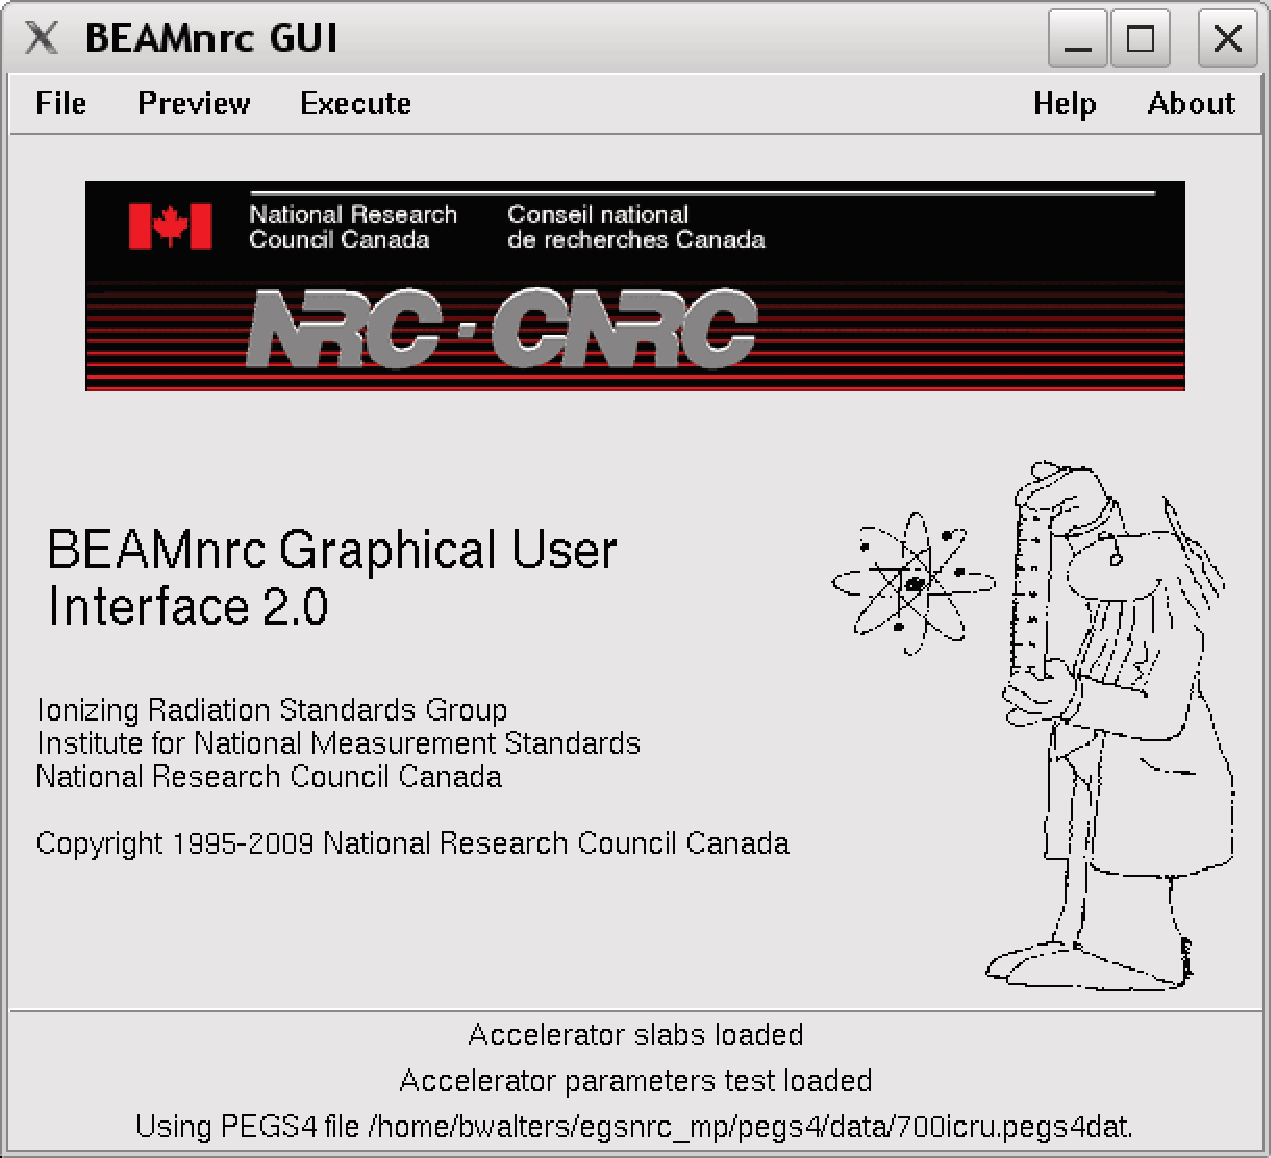
\includegraphics[width=12cm]{figures/gui_main_window}

The main window of the BEAM GUI.
\end{center}
\end{figure}


\vfill
\copyright NRC Canada, 2015
\end{center}

\setlength{\baselineskip}{0.2cm}
\newpage

\pagestyle{fancy}
\pagenumbering{arabic}
\setcounter{page}{2}

\newpage

\begin{center}
\begin{Large}
{\bf Abstract}
\end{Large}
\end{center}
This document is intended for anyone who will be making changes to the
BEAM or DOSXYZ GUI code.  It contains variable naming conventions, a list of
procedures and what they do, and a flow diagram of how they interact
with each other.
\vspace*{4cm}\\

\tableofcontents

\setlength{\baselineskip}{0.5cm}

\newpage

%\pagestyle{myheadings}

\chapter{BEAM GUI}

{\sffamily
\section{Introduction}
}


Currently the working source code for the GUIs are stored in
{\tt \$OMEGA\_HOME/progs/gui/beam} and {\tt
\$OMEGA\_HOME/progs/gui/dosxyz}.  They are written in Tcl/Tk.  On this
system, the
versions available are Tk version 4.1 and Tcl version 7.5 with wish
version 4.1.  These are older versions.  Note that Tcl/Tk is not always
backward compatible, but is more backward than forward compatible.  We
also have wish8.0 (neotcl8.0) but the ``wish'' symbolic link points to wish4.1.
At this time, the GUIs are not portable to Windows or Mac because when
directory trees are specified I did not always use the 'file join' command but
simply put in forward slashes, '/'.  This doesn't matter because BEAM
only runs on UNIX-based systems.  It might be fun to try it out though...

\section{Tcl/Tk Notes}

Tcl is a scripting language and is similar in syntax to C-shell
scripts.  When referencing a variable which has been set (using
{\tt set var 5} for example), the dollar sign is used:
{\tt set newvar \$var}.

Tcl does just about everything in strings.  '=' is not used.  If you
want to set a value, you have to use {\tt set var 6}.
It manages to regard {\tt \$var} as an integer if for loops, but if you
want to do any
math with it you have to use the 'expr' command, for example,
{\tt set newvar [expr 5 * \$var]}.

One problem I encountered was reading an integer from a file.  Say that
integer is 3, and I read it as 'var' then I want to compare it:
{\tt if \{ \$var == 3 \} \{ ...}
This statement may come back as false if there are trailing
spaces in the file.  To fix this, use {\tt set var [expr \$var]}.

Arrays can be created in Tcl, but the important note is that the index
of the array is regarded as a string, not as an integer.  For example,
an array can be \verb+array(3)+ or \verb+array(colour)+.  Two-dimensional arrays
can only be emulated by using \verb+array(2,1)+ for example, which would NOT
be the same thing as \verb+array(2, 1)+.

\subsection{Previews}

The canvas widget is used for all previews.  A main canvas is put on the
window first.  If there is more than one perspective to be shown, new
canvas widgets are created, then placed on the main canvas after being
drawn on.  Otherwise the drawing is done on the main canvas.
The CM is drawn on first, in the appropriate scale.  Then four
rectangles are drawn on the canvas to cover up the parts of the CM
drawing that stray beyond the drawing region (procedure coverup).  Then
the axes are drawn on (procedure draw\_axes).

The preview of the entire accelerator (draw\_accel) either uses only the xz
cross-sectional views for each component or the yz cross-sectional
views.  For that reason, all xz
cross-section procedures are named {\sf add\_\$cmname} and all yz
cross-section procedures are named {\sf add\_\$cmname\_yz}.  Of course,
if the CM is radially symmetric, like SLABS CONS3R CONESTAK FLATFILT and
CHAMBER, there is no difference between yz and xz cross-sections so
there's only one precedure, {\sf add\_\$cmname}, for both.  The xy
cross-section procedure is {\sf add\_\$cmname\_xy}.  For the MLC
preview, since the leaves could be
parallel or perendicular to x, the procedured are names {\sf
add\_MLC\_sides} and {\sf add\_MLC\_ends} and are treated as a special
case.

\subsection{Translating an (x,y) point onto canvas coordinates}

Let the real axes have ranges ($x_{min}$,$x_{max}$) and
($y_{min}$,$y_{max}$) and let the
canvas be $n\times n$.  Then for the x coordinate,
$$
x_c=mx_r+b
$$
Using the translation of the origin of the real coordiante system,
$(0,0)_c\rightarrow (x_{min},y_{min})_r$,
$$
x_c=m x_{min}+b=0
$$
so that $b=-m x_{min}$.  The using the translation of the maximum,
$(n,n)_c\rightarrow (x_{max},y_{max})_r$,
$$
x_c=m x_{max}+b=m x_{max}-m x_{min}=n
$$
so that $m=n/(x_{max}-x_{min})$.  Putting it all together,
$$
x_c=n\frac{(x_r-x_{min})}{(x_{max}-x_{min})}
$$
Note that the origin on the canvas is in the upper left-hand corner.
To shift the entire graph on the canvas to an origin of (l,m) simply add
these to x and y:
$$
x_c=n\frac{(x_r-x_{min})}{(x_{max}-x_{min})}+l
$$
and similarly for the y-coordinate,
$$
y_c=n\frac{(y_r-y_{min})}{(y_{max}-y_{min})}+m
$$

\section {The BEAM GUI}


\section{Tcl/Tk Files for the BEAM GUI}

The files required for the GUI are the following:

\begin{enumerate}
\item {\tt beam\_gui} is the main script.  It pops up the initial window.
The main window presents the user with four options,

\begin{itemize}
\item load a previous accelerator -- allows the user to browse their
.module files to select an accelerator to work with.

\item specify a new accelerator -- allows the user to create a new
accelerator by specifying the CMs they intend to use as well as giving
them identifying names.

\item load a previous input file -- allows the user to browse their home
directory for a previously made input file.  If an accelerator has been
loaded, an attempt is made to start the browser off in the directory
corresponding to the accelerator selected.  If that is not possible, or
if an accelerator has not yet been loaded, the browser starts in the
{\tt \$home/egs4} directory.

If an accelerator has not been loaded and an input file is selected, an
attempt is made to load the appropriate accelerator based on the
directory tree.

\item save input parameters as... -- allows the user to browse
directories and specify an input file name to save the input parameters
as.
\end{itemize}
\begin{enumerate}
\item {\sf proc get\_beam\_user\_defaults \{\}} reads in default maximum
and minimum parameter values from {\tt beam\_user\_macros.mortran}.
\item {\sf about\_BEAM\_GUI \{\}} pops up a window describing the origin
of the GUI.
\item {\sf about\_BEAM \{\}} pops up a window describing the origin
of BEAM.
\item {\sf exit\_prompt \{\}} puts an ``Are you sure'' dialog up before exiting.
\end{enumerate}

\item {\tt beam\_params.tcl} contains parameter settings for the GUI,
like parameter names
and initial values and the various options for those parameters with
multiple options.  There are no procedures in this file.

\item {\tt create\_accel.tcl} contains procedures which allow the user
to build a new
accelerator and procedures to display it or previously built accelerator
on the screen.
\begin{enumerate}
\item {\tt specify\_new\_module \{\}} calls {\sf create\_accel} after checking
whether an accelerator is already loaded and prompting to discard it if
necessary.  It is called from the main File menu, ``specify a new
accelerator''.
\item {\sf popup\_cm\_window \{\}} creates a toplevel window to hold the
labels and buttons which display the selected CMs.
\item {\sf update\_popup \{\}} is called when a new CM is added or when a
module file is finished loading.  It puts the CM name, identifier and
Edit button on the popup window.
\item {\sf edit\_cm \{ id index \}} is called when the ``Edit'' button is
pressed for a CM.  id is the chronological CM number and index is cm\_type(\$id)
The Z-coordinate of the end of the previous CM is calculated by calling
{\sf get\_zmax} (in {\tt draw\_accel.tcl}).  That number is then passed
to the CM being edited so that the user knows where the last CM ended.
\item {\sf create\_accel \{\}} is the procedure used to pop up a window so
that the user can select form the available CMs, give it an identifier
name, and add it to the popup window using {\sf add\_cm}.
\item {\sf seeifsaved \{\}} is used when the user was working on a new
accelerator and tries to exit without saving.  It prompts with an ``Are
you sure?''
\item {\sf put\_cm\_in\_textbox \{\}} is used with a double-click binding
with {\sf create\_accel}, to automatically insert a CM name into the selected
textbox beside the list.
\item {\sf add\_cm \{\}} is used to add a CM to the list selected for the
accelerator.  It is called by {\sf create\_accel} and in turn calls
{\sf update\_popup}.  It sets the variables for selected CMs.
\end{enumerate}

\item {\tt query\_filename.tcl} contains the procedure for browsing a
directory tree for a file.
\begin{enumerate}
\item {\sf query\_filename \{next\_proc\_name dir ext\}} is the main
procedure. {\tt next\_proc\_name} is the procedure to follow when the
``OK'' button is pressed,  {\tt dir} is the starting directory for the search,
and {\tt ext} is a file extension, which serves as a filter.
\item {\sf call\_next\_proc \{ next\_proc\_name \}} is the procedure called
when the ``OK'' button is clicked.  It calls {\tt next\_proc\_name}.
\end{enumerate}

\item {\tt browser.tcl} is similar to {\sf query\_filename} but does not use a
filter and always starts in the user's egs4 directory.  {\tt next\_proc\_name}
is always one of the four 'set\_*' listed below.
\begin{enumerate}
\item {\sf browse \{next\_proc\_name\}} pops up a browser with no filter.
\item {\sf set\_spcnam15 \{\}} sets {\tt spcnam15} to the file selected
in browse.
\item {\sf set\_spcnam21 \{\}} sets {\tt spcnam21} to the file selected
in browse.
\item {\sf set\_spcnam31 \{\}} sets {\tt spcnam31} to the file selected
in browse.
\item {\sf set\_spec\_file \{\}} sets {\tt spec\_file} to the file
selected in browse.
\end{enumerate}

\item {\tt save\_module.tcl} contains procedures for saving a module file
(some of which are also used for saving an input file).
\begin{enumerate}
\item {\sf save\_module \{\}} is the procedure for saving an accelerator.  It
calls query\_filename to obtain a module filename, with arguments
{\tt DoesModFileExist egs4/beam/spec\_modules module}.
\item {\sf DoesModFileExist \{ tree filename \}} checks whether the module
file selected already exists, and if so, it calls {\sf overwrite\_prompt} to
prompt the user before overwriting.  {\sf save\_proc} is {\sf
save\_mod\_file} and type is 'mod', used in {\sf overwrite\_prompt}.
\item {\sf save\_mod\_file \{tree filen\}} saves the module file to the file
{\tt tree/filen}.
\item {\sf overwrite\_prompt \{tree filename save\_proc type\}} prompts the
user as to whether it's okay to overwrite the file {\tt tree/filename}, if it
already exists.  type is either 'mod' or 'inp', for module or input.
\end{enumerate}

\item {\tt load\_input2.tcl} contains procedures for loading a previously made
input file.
\begin{enumerate}
\item {\sf load\_input \{\}} attempts to locate the appropriate starting
directory based on the module file loaded, if any, and then calls {\sf
query\_filename} with {\sf set\_inp\_file} as the {\tt next\_proc\_name}.
\item {\sf set\_inp\_file \{tree filen\}} sets the input file name
{\tt inp\_file} to that selected in {\sf query\_filename}, {\tt
tree/filen}.  If there
is no accelerator loaded, however, it tries to locate the appropriate
module file.  If it can't find it, the user is alerted that an
accelerator must be loaded first.
\item {\sf get\_val \{ data varname i \}} scans the string data for the
first number in the line and sets varname(\$i) to this value.
\item {\sf get\_str \{ data varname i \}} gets a string from data and
trims the whitespace off either end, and sets varname(\$i) to this value.
\item {\sf read\_input \{\}} reads in the input file.  It uses the
information loaded from the module file to read the CM parameters.
\end{enumerate}

\item {\tt load\_module.tcl} contains procedures to load a previously defined
accelerator.
\begin{enumerate}
\item {\sf load\_old\_module \{\}} checks whether an accelerator is already
loaded, and if so, prompts the user as to whether it should be
discarded.  It calls {\sf query\_filename} with {\sf set\_mod\_file} as the next
procedure.
\item {\sf set\_mod\_file \{tree filen\}} sets {\tt mod\_file} to {\tt
tree/filen}, then calls {\sf load\_module} to read in the information.
\item {\sf load\_module \{\}} reads in the accelerator information, \ie~
the CM names and identifiers ({\tt cm\_name(i), cm\_ident(i)}).
\end{enumerate}

\item {\tt pegs4.tcl} contains procedures for loading a PEGS4 file.
\begin{enumerate}
\item {\sf get\_pegs4file \{\}} pops up a window to select the PEGS4
file.  The user has to select it by browsing (which calls {\sf
query\_filename}).
\item {\sf set\_pegs4filename \{ tree filename \}} sets the {\tt
pegs4file} to {\tt tree/filename} and configures the label that displays
the directory it was selected from.
\item {\sf check\_pegs4file \{\}} If the file was selected from the {\tt
HEN\_HOUSE}, the user's home directory is searched for a matching
file.  If found, a dialog box appears informing the user that they'll
have to reselect the file in their home directory, since BEAM will
search this first.
\end{enumerate}

\item {\tt set\_main\_inputs.tcl}
\begin{enumerate}
\item {\sf set\_main\_inputs \{\}} first checks whether an accelerator has
been loaded and if not it pops up an info window to tell the user to
load or create one first before the main inputs can be set.  Otherwise,
it pops up the main window for setting main inputs, which puts the
parameter labels ({\tt names(\$i)}) and text boxes/option menus up on
the window.  Any parameters which are off-shoots of these are dealt with
on a child window.
\item {\sf set\_medium \{ iopt \}} sets the medium ({\tt values(2)}) to
{\tt medium(iopt)} and configures the option menu to show this value.
\item {\sf make\_menu\_button \{i w\}} creates an option menu for parameter i
on frame w (left or right side of the main window).  The command
{\tt set\_value} is associated with each option.
\item {\sf make\_text\_box \{i w\}} creates a text entry box for parameter i
on frame w (left or right side of the main window).
\item {\sf set\_value \{io iopt w\}} is used with the option menu
command.  {\tt io}
is the parameter index (\ie~{\tt names(\$io)}), {\tt iopt} is the index
of the option selected and w is the menu widget it came from.
Generally, this prcedure sets the value of the parameter to that
selected by the user and configures the option menu widget to display
this choice.  For those parameters which require setting further
parameter values, another procedure is called from here.  These are
listed below.
\item {\sf set\_nbrem \{\}} asks the user for the number of brem photons, when
uniform brem splitting is selected, and also FS, SSD, NMIN when
selective brem splitting is selected.  In both cases, gives the Russian
Roulette option menu.
\item {\sf set\_special\_N \{\}} is used with the special case of IWATCH; it
asks for the history at which to set IWATCH to 2.
\item {\sf set\_scoring\_options \{ nplanes \}} is an offshoot of the number
of scoring planes (nplanes).  It gets {\tt IPLANE\_TO\_CM} and the number of
scoring zones.
\item {\sf get\_zone\_marks \{ w izone \}} is called from
{\sf set\_scoring\_options} to get the zone marks after the number of zones in
input.
\item {\sf set\_28\_3 \{ i w label \}} sets the value of
{\tt values(28,3,\$i)} to {\tt \$label} and configures {\tt \$w.inp} to display
it.  This value is the zone type
and is called from {\sf set\_scoring\_options}.
\item {\sf set\_itdose\_on \{\}} is called when dose calculations are
selected.  It asks for the contaminant type, the CM at which to identify
it as contaminant, and the number of inclusive and exclusive bit filters
desired.
\item {\sf configure\_menu \{ w i j k \}} configures widget {\tt
\$w.inp} to display
{\tt \$options(\$i,\$j,\$k)} on it.  It is exclusively for use in
set\_itdose\_on to set the contaminant type.
\item {\sf set\_ln\_exc \{\}} is called when the number of dose components
with exclusive bit filters are defined.  It uses radiobuttons to select bits.
\item {\sf set\_ln\_inc \{\}} is called when the number of dose components
with inclusive bit filters are defined.  It uses radiobuttons to select bits.
\item {\sf set\_force\_options \{\}} is called when photon forcing is set to
on.  A window pops up asking for the four options associated with this
parameter.
\item {\sf set\_ifluor\_options \{ level \}} is called when x-ray fluorescence
is set to on.  It asks for the effective Z, from and to regions.
\item {\sf set\_src\_options \{ iopt \}} is called when source {\tt iopt} is
selected.  Note that iopt does not follow the numbering assigned to the
sources in the user manual but are chronological in the same order as in
the manual.  The user is asked to set the source options associated with
the source selected (number of options and option names are set in
{\tt beam\_params.tcl}).  Any further options, such as spectrum files
or beam energies, are also there.
\item {\sf get\_s9vals \{ w \}} pops up a window with text boxes so that the
user can input the discrete probabilities for source 9.
\item {\sf set\_ioutsp \{label\}} is called when the variable ioutsp is set on
the main source options window.  It configures the option menu to
display the new value and sets the parameter value.
\end{enumerate}

\item {\tt save\_input.tcl} contains procedures to save an input file.
\begin{enumerate}
\item {\sf save\_input \{\}} is the main procedure for saving an input file.  It
calls {\sf query\_filename} to obtain an input filename, with arguments
{\tt DoesModFileExist \$inp\_file\_dir egs4inp}.  If {\tt
\$inp\_file\_dir} doesn't
exit, it asks the user if they want to create it.
\item {\sf DoesInpFileExist \{\}} checks to see whether the file exists.  If
it does, it calls {\sf overwrite\_prompt}.  It then calls {\sf save\_inp\_file}.
\item {\sf save\_inp\_file \{tree filen\}} sets the variable {\tt inp\_file} to
{\tt tree/filen}, then calls {\sf create\_file} to generate the file.
\end{enumerate}

\item {\tt help.tcl} contains all of the help windows.  The first procedure is
{\sf help}, which calls {\sf help\_dialog} to pop up a window to display the help
text for the main input parameters.  The second procedure is
{\sf help\_srcopts}, which calls {\sf help\_gif} to pop up a window to
display the
gif file and help text for the sources.  The rest of the procedures have
names that start with {\sf help\_} and the rest of the name is (hopefully)
obvious.

\item {\tt new\_create\_file.tcl} contains the procedures used to write an
input file.
\begin{enumerate}
\item {\sf create\_file \{ file \}} writes the main parameters and the
parameters defined for the selected CMs to a file in the specified
format.  It is called from {\sf save\_inp\_file}.
\end{enumerate}

\item {\tt misc.tcl} contains dialog boxes and macro-ish procedures that are
used alot in the CM procedures (ecut, pcut, etc.).
\begin{enumerate}
\item {\sf tk\_dialog \{ w title text bitmap default args \}} overrides the tk
pre-made procedure.  I increased the width of the box and changed the
font to helvetica.
\item {\sf help\_dialog \{ w title text bitmap default args \}} creates a
window with a scrollbar to display {\tt text}.  The scrollbar is required
for those help texts with more than 30 lines.
\item {\sf help\_gif \{ w text iconfile \}} creates a window with {\tt
iconfile} (a gif file) displayed on the left and {\tt text} on the right.
It is used for the source helps and the CM helps.
\item {\sf get\_1\_default \{ name top text \}} is used when
there is one default value defined in {\tt \$name\_macros.mortran} and
displays it at the top of the main edit window for all CMs.
\item {\sf get\_2\_defaults \{ name top str1 text1 str2 text2 \}} is used when
there are two default values defined in {\tt \$name\_macros.mortran} and
displays them at the top of the main edit window for all CMs.
\item {\sf add\_rmax\_square \{ w index \}} adds the block of helpbutton, label,
textbox for {\tt RMAX\_CM} for a square CM.
\item {\sf add\_rmax\_rad \{ w index \}} adds the block of helpbutton, label,
textbox for {\tt RMAX\_CM} for a radially symmetric CM.
\item {\sf add\_title \{ w index \}} adds the block of helpbutton, label,
textbox for {\tt TITLE}.
\item {\sf add\_zmin \{ w index \}} adds the block of helpbutton, label,
textbox for {\tt ZMIN}.
\item {\sf add\_ecut \{ w index \}} adds the block of helpbutton, label,
textbox for {\tt ECUT}.
\item {\sf add\_pcut \{ w index \}} adds the block of helpbutton, label,
textbox for {\tt PCUT}.
\item {\sf add\_dose \{ w index \}} adds the block of helpbutton, label,
textbox for {\tt DOSE\_ZONE}.
\item {\sf add\_latch \{ w index \}} adds the block of helpbutton, label,
textbox for {\tt LATCH}.
\item {\sf add\_material \{ w index \}} adds the block of helpbutton, label,
textbox for {\tt MATERIAL}.
\item {\sf set\_material \{ w iopt index \} } sets the material for the
{\sf add\_material} option menu.
\end{enumerate}

\item {\tt change\_color\_scheme.tcl} contains procedures for the user
to change the colour scheme for drawing.  A default colour scheme is set
up in beam\_gui, but greyscale can be selected here, and by clicking on
a colour swatch the user can alter the rgb values of a colour using
scale widgets.
\begin{enumerate}
\item {\sf change\_color\_scheme \{\}} pops up a window with the colours
on 10x10 canvases on a grid with the materials they correspond to.
\item {\sf change\_to\_colour \{\}} resets colorlist when one of the
radiobuttons, colour or greyscale, is selected.
\item {\sf change\_color \{ parent\_w i \}} pops up a window with the
rgb scale widgets (or with one scale widget if greyscale selected) and a
canvas to display the colour.
\item {\sf update\_palette \{ parent\_w col value \}} changes the colour
of the canvas on the window with the rgb scales when the scales are moved.
\item {\sf set\_color \{ parent\_w i \}} is called when the Accept button
is selected on the window with the rgb scales; it sets the new value for
the colour in colorlist (uses lrm).
\item {\sf lrm \{ list pos item \}} replaces element at pos in list with
item.
\end{enumerate}

\item {\tt draw\_accel.tcl} contains procedures for the preview of the
entire accelerator, xz cross-section.
\begin{enumerate}
\item {\sf draw\_accel \{\}} pops up a window with a colour legend and
buttons on the left and a canvas in scrollbars on the right.  The colour
swatches on the legend can be clicked to edit the colour scheme; only
the materials used are shown.
\item {\sf redraw\_accel \{\}} draws the accelerator to scale on the
canvas.
\item {\sf change\_accel\_range \{\}} pops up a window with x and z
ticks, zoom scales and ranges so that the user can customize the plot.
\item {\sf get\_zmax \{ id \}} finds the maximum z of the CM at position
id in the accelerator.
\end{enumerate}

\item {\tt slabs.tcl}
\begin{enumerate}
\item {\sf init\_SLABS \{ id \}} initializes the parameters for SLABS, the CM
at index \$id.
\item {\sf read\_SLABS \{ fileid id \}} reads in the SLABS section of an input
file \$fileid, to be stored as the CM at index \$id.
\item {\sf edit\_SLABS \{ id \}} pops up the window for editing SLABS
parameters for the CM at index \$id.
\item {\sf define\_nslabs \{ id \}} is an offshoot window to define the layers.
\item {\sf write\_SLABS \{ fileid id \}} writes the parameter set for the SLABS
CM at index \$id to file \$fileid.  It is called from {\sf create\_file}.
\item {\sf show\_SLABS \{ id \}} pops up a window in which to display
the canvas for the preview of the CM, and assigns colours to the media
used.
\item {\sf draw\_SLABS \{ id \}} creates the canvas (or canvasses,
depending on the CM) required for the preview.
\item {\sf add\_SLABS \{ id xscale zscale xmin zmin l m parent\_w \}}
draws the graphic on parent\_w.  l is the space on the left of the graph
and m is the space from the top of the graph.  xmin and zmin are the
minimum axis ranges, xscale and zscale are the scale factors for x and
z.
\item {\sf coverup \{ l m width canvas \}} puts four white rectangles on
canvas to cover up the drawing parts that go beyond the drawing area.
width is the width and height of the drawing area, l and m are as above.
\item {\sf add\_axes \{ pair n1 n2 l m width a b c d scale1 scale2
canvas \}} draws the axes on canvas.  pair can be xy, xz or yz.  n1 and
n2 are the number of ticks to put on the 1st and 2nd axis respectively.
width, l and m are as above.  a, b, c and d are the pairs of min and max
values for the 1st and 2nd axes, respectively.
\item {\sf change\_cm\_range \{ id parent xyz \}} pops up a window to change the
axis ranges and the number of ticks on the axes.  Used by ALL CM
previews.  parent is the canvas that's being changed and is used when
Apply is selected to redraw based on these changes.  xyz can be xyz, xy,
xz, or yz, depending on how many perspectives are displayed.
\end{enumerate}

Unless explicitly stated, the init, read, edit, write, show, draw and
add procedures have
a description similar to that stated in SLABS.

\item {\tt cons3r.tcl}
\begin{enumerate}
\item {\sf init\_CONS3R \{ id \}}
\item {\sf read\_CONS3R \{ fileid id \}}
\item {\sf edit\_CONS3R \{ id \}}
\item {\sf define\_nnode \{ id \}} pops up a window for the definition
of the points used in this CM.
\item {\sf write\_CONS3R \{ fileid id \}}
\item {\sf show\_CONS3R \{ id \}}
\item {\sf draw\_CONS3R \{ id \}}
\item {\sf add\_CONS3R \{ id xscale zscale xmin zmin l m parent\_w \}}
\end{enumerate}

\item {\tt conestak.tcl}
\begin{enumerate}
\item {\sf init\_CONESTAK \{ id \}}
\item {\sf read\_CONESTAK \{ fileid id \}}
\item {\sf edit\_CONESTAK \{ id \}}
\item {\sf disable\_if\_off \{ id \}} is used to disable the input area for the
outer wall if it has been selected as not present.  It is called when
the checkbutton is clicked and uses the variable owall\_conestak(\$id).
\item {\sf define\_conestak\_props \{ id \}} pops up a window for
defining the properties of the layers, inside and outside.
\item {\sf define\_conestak\_dim \{ id \}} pops up a window for defining
the dimensions of each layer (thickness, top radius, back radius).
\item {\sf write\_CONESTAK \{ fileid id \}}
\item {\sf show\_CONESTAK \{ id \}}
\item {\sf draw\_CONESTAK \{ id \}}
\item {\sf add\_CONESTAK \{ id xscale zscale xmin zmin l m parent\_w \}}
\end{enumerate}

\item flatfilt.tcl
\begin{enumerate}
\item {\sf init\_FLATFILT \{ id \}}
\item {\sf read\_FLATFILT \{ fileid id \}}
\item {\sf edit\_FLATFILT \{ id \}}
\item {\sf define\_layers \{ id \}}: if there is more than one window
required (more than 9 layers), a child pops up to hold buttons for
``Edit layers 1-9, 10-18, etc.'', which connects to procedure
{\sf define\_layer\_window} for those layers.  Otherwise we go directly to
{\sf define\_layer\_window} for all layers.
\item {\sf set\_flatfilt\_button\_color \{ id ilayer start end \}} determines
whether all of the necessary parameters have been set for layers {\tt start}
to {\tt end}, corresponding to button {\tt ilayer}.  If they haven't, the button
colour is set to red, otherwise black.
\item {\sf define\_layer\_window \{ id \}} pops up a window with thickness and
number of cones in the layer for each layer.  A ``Define conical sections $>>$''
button leads to {\sf define\_cones}.
\item {\sf define\_cones \{ parent id indx \}} pops up a window for layer
{\tt indx} so that the user can set the geometry and properties of each cone
in the layer.
\item {\sf write\_FLATFILT \{ fileid id \}}
\item {\sf show\_FLATFILT \{ id \}}
\item {\sf draw\_FLATFILT \{ id \}}
\item {\sf add\_FLATFILT \{ id xscale zscale xmin zmin l m parent\_w \}}
\end{enumerate}

\item jaws.tcl
\begin{enumerate}
\item {\sf init\_JAWS \{ id \}}
\item {\sf read\_JAWS \{ fileid id \}}
\item {\sf edit\_JAWS \{ id \}}
\item {\sf define\_jaws \{ id \}} pops up a window for defining the
geometric and material properties of each set of paired bars.
\item {\sf write\_JAWS \{ fileid id \}}
\item {\sf show\_JAWS \{ id \}}
\item {\sf draw\_JAWS \{ id \}}
\item {\sf add\_JAWS \{ id xscale zscale xmin zmin l m parent\_w \}}
\item {\sf add\_JAWS\_yz \{ id yscale zscale ymin zmin l m parent\_w \}}
\end{enumerate}

\item circapp.tcl
\begin{enumerate}
\item {\sf init\_CIRCAPP \{ id \}}
\item {\sf read\_CIRCAPP \{ fileid id \}}
\item {\sf edit\_CIRCAPP \{ id \}}
\item {\sf define\_circapp \{ id \}} pops up a window for defining
geometry and material properties of each scraper.
\item {\sf write\_CIRCAPP \{ fileid id \}}
\item {\sf show\_CIRCAPP \{ id \}}
\item {\sf draw\_CIRCAPP \{ id \}}
\item {\sf add\_CIRCAPP \{ id xscale zscale xmin zmin l m parent\_w \}}
\item {\sf add\_CIRCAPP\_xy \{ id xscale yscale xmin ymin l m parent\_w \}}
\item {\sf add\_CIRCAPP\_yz \{ id yscale zscale ymin zmin l m parent\_w \}}
\end{enumerate}

\item applicat.tcl
\begin{enumerate}
\item {\sf init\_APPLICAT \{ id \}}
\item {\sf read\_APPLICAT \{ fileid id \}}
\item {\sf edit\_APPLICAT \{ id \}}
\item {\sf define\_applicat \{ id \}} pops up a window for defining
geometry and material properties of each scraper.
\item {\sf write\_APPLICAT \{ fileid id \}}
\item {\sf show\_APPLICAT \{ id \}}
\item {\sf draw\_APPLICAT \{ id \}}
\item {\sf add\_APPLICAT \{ id xscale zscale xmin zmin l m parent\_w \}}
\item {\sf add\_APPLICAT\_xy \{ id xscale yscale xmin ymin l m parent\_w \}}
\item {\sf add\_APPLICAT\_yz \{ id yscale zscale ymin zmin l m parent\_w \}}
\end{enumerate}

\item pyramids.tcl
\begin{enumerate}
\item {\sf init\_PYRAMIDS \{ id \}}
\item {\sf read\_PYRAMIDS \{ fileid id \}}
\item {\sf edit\_PYRAMIDS \{ id \}}
\item {\sf define\_pyramids \{ id \}} pops up a window for defining
geometry and material properties of each layer.
\item {\sf set\_grid\_material \{ w iopt index \}} configures the option
menu {\tt w} in the grid on the window created in {\sf
define\_pyramids} to a value of {\tt cmval(index)} and sets {\tt
cmval(index)} to {\tt medium(iopt)}.
\item {\sf write\_PYRAMIDS \{ fileid id \}}
\item {\sf show\_PYRAMIDS \{ id \}}
\item {\sf draw\_PYRAMIDS \{ id \}}
\item {\sf add\_PYRAMIDS \{ id xscale zscale xmin zmin l m parent\_w \}}
\item {\sf add\_PYRAMIDS\_yz \{ id yscale zscale ymin zmin l m parent\_w \}}
\end{enumerate}

\item chamber.tcl
\begin{enumerate}
\item {\sf init\_CHAMBER \{ id \}}
\item {\sf read\_CHAMBER \{ fileid id \}}
\item {\sf edit\_CHAMBER \{ id \}}
\item {\sf define\_chamber\_top\_props \{ id \}} pops up a window for
defining the material and properites of each layer in the top of the chamber.
\item {\sf define\_chamber\_bot\_props \{ id \}} pops up a window for
defining the material and properites of each layer in the bottom of the
chamber.
\item {\sf define\_chamber\_props \{ id \}} pops up a window for
defining the material and properites of each layer in the central region
of the chamber.
\item {\sf set\_button\_color \{ id i \}} sets the ``edit layer'' button to
red if the thickness or material have not been defined for layer i.
\item {\sf edit\_group\_thick \{ id \}} is used to set the thicknesses of
groups when defining the chamber as groups.
\item {\sf edit\_layer \{ id layer \}}
\item {\sf calculate\_distance \{ id layer \}} is used to calculate the distance
from the top of chamber to the current layer.
\item {\sf set\_same\_as\_layer \{ id layer \}} is used to set the current layer
to have the same values as \$sameaslayer (a global variable).
\item {\sf write\_CHAMBER \{ fileid id \}}
\item {\sf show\_CHAMBER \{ id \}}
\item {\sf draw\_CHAMBER \{ id \}}
\item {\sf add\_CHAMBER \{ id xscale zscale xmin zmin l m parent\_w \}}
\end{enumerate}

\item mirror.tcl
\begin{enumerate}
\item {\sf init\_MIRROR \{ id \}}
\item {\sf read\_MIRROR \{ fileid id \}}
\item {\sf edit\_MIRROR \{ id \}}
\item {\sf calc\_mirror\_angle \{ id \}} is used to calculate the angle of the
mirror given the geometry specified.
\item {\sf define\_mirrors \{ id \}} pops up a window to define the
thickness and material properties of each layer in the mirror.
\item {\sf write\_MIRROR \{ fileid id \}}
\item {\sf show\_MIRROR \{ id \}}
\item {\sf draw\_MIRROR \{ id \}}
\item {\sf add\_MIRROR \{ id xscale zscale xmin zmin l m parent\_w \}}
\end{enumerate}

\item mesh.tcl
\begin{enumerate}
\item {\sf init\_MESH \{ id \}}
\item {\sf read\_MESH \{ fileid id \}}
\item {\sf edit\_MESH \{ id \}}
\item {\sf write\_MESH \{ fileid id \}}
\item {\sf show\_MESH \{ id \}}
\item {\sf draw\_MESH \{ id \}}
\item {\sf add\_MESH \{ id xscale zscale xmin zmin l m parent\_w \}}
\item {\sf add\_MESH\_xy \{ id xscale yscale xmin ymin l m parent\_w \}}
\end{enumerate}

\item xtube.tcl
\begin{enumerate}
\item {\sf init\_XTUBE \{ id \}}
\item {\sf read\_XTUBE \{ fileid id \}}
\item {\sf edit\_XTUBE \{ id \}}
\item {\sf define\_xtube \{ id \}} pops up a window to define the
thickness and material properties of each layer in the x-ray tube.
\item {\sf write\_XTUBE \{ fileid id \}}
\item {\sf show\_XTUBE \{ id \}}
\item {\sf draw\_XTUBE \{ id \}}
\item {\sf add\_XTUBE \{ id xscale zscale xmin zmin l m parent\_w \}}
\end{enumerate}

\item sidetube.tcl
\begin{enumerate}
\item {\sf init\_SIDETUBE \{ id \}}
\item {\sf read\_SIDETUBE \{ fileid id \}}
\item {\sf edit\_SIDETUBE \{ id \}}
\item {\sf define\_sidetube \{ id \}} pops up a window to define the
outer radius and material properties of each layer in the sidetube.
\item {\sf write\_SIDETUBE \{ fileid id \}}
\item {\sf show\_SIDETUBE \{ id \}}
\item {\sf draw\_SIDETUBE \{ id \}}
\item {\sf add\_SIDETUBE \{ id xscale zscale xmin zmin l m parent\_w \}}
\item {\sf add\_SIDETUBE\_xy \{ id xscale yscale xmin ymin l m parent\_w \}}
\end{enumerate}

\item mlc.tcl
\begin{enumerate}
\item {\sf init\_MLC \{ id \}}
\item {\sf read\_MLC \{ fileid id \}}
\item {\sf edit\_MLC \{ id \}}
\item {\sf define\_leaves \{ id \}} pops up a window to define the
size of the leaves in the mlc, in groups.
\item {\sf save\_mlc \{ id \}} is used when leaving {\sf
define\_leaves}.  It checks that an error hasn't been made when defining
the leaves, and if so it informs the user.
\item {\sf add\_mlc\_row \{ id \}} is invoked when ``Add a row'' is
clicked on the window in {\sf define\_leaves}.  It adds a new group to
the bottom of the list.  If all the leaves are currently defined, it
does not allow a new group.
\item {\sf write\_MLC \{ fileid id \}}
\item {\sf show\_MLC \{ id \}}
\item {\sf draw\_MLC \{ id \}}
\item {\sf add\_MLC\_ends \{ id xscale zscale xmin zmin zmax l m parent\_w \}}
\item {\sf add\_MLC\_sides \{ id xscale zscale xmin zmin zmax l m parent\_w \}}
\item {\sf add\_MLC\_xy \{ id xscale yscale xmin ymax l m parent\_w \}}
\end{enumerate}

\item block.tcl
\begin{enumerate}
\item {\sf init\_BLOCK \{ id \}}
\item {\sf read\_BLOCK \{ fileid id \}}
\item {\sf edit\_BLOCK \{ id \}}
\item {\sf define\_block \{ id \}} is called from {\sf edit\_BLOCK}; it
pops up a window  to set the number of points which define each subregion.
\item {\sf define\_points \{ j id \}} is called from {\sf
define\_block}; it allows the user to set the (x,y) points for each subregion.
\item {\sf check\_block\_angles \{ id subreg \}}
\item {\sf cross \{ x1 y1 x2 y2 x3 y3 \}}
\item {\sf write\_BLOCK \{ fileid id \}}
\item {\sf show\_BLOCK \{ id \}}
\item {\sf draw\_BLOCK \{ id \}}
\item {\sf add\_BLOCK \{ id xscale zscale xmin zmin l m parent\_w \}}
\item {\sf add\_BLOCK\_xy \{ id xscale yscale xmin ymax l m parent\_w \}}
\item {\sf print\_canvas \{ w \}} pops up a window so the user can
choose colour or black and white, portrait or landscape, and print to a
file or to a printer.
\item {\sf print\_cmd \{ w \}} executes the print command based on what
the user chose.
\end{enumerate}

\item arcchm.tcl
\begin{enumerate}
\item {\sf init\_ARCCHM \{ id \}}
\item {\sf read\_ARCCHM \{ fileid id \}}
\item {\sf edit\_ARCCHM \{ id \}}
\item {\sf define\_arcchm\_props \{ id \}} is called from {\sf edit\_ARCCHM}; it
pops up a window  to define the properties of each ion chamber and septum.
\item {\sf write\_ARCCHM \{ fileid id \}}
\item {\sf show\_ARCCHM \{ id \}}
\item {\sf draw\_ARCCHM \{ id \}}
\item {\sf add\_ARCCHM \{ id xscale zscale xmin zmin l m parent\_w \}}
\item {\sf add\_ARCCHM\_yz \{ id yscale zscale ymin zmin l m parent\_w \}}
\end{enumerate}

\end{enumerate}

The last 15 files are specifically for the CMs they are named for.  The
{\sf init\_\$name}, {\sf read\_\$name}, {\sf edit\_\$name}, {\sf
write\_\$name}, {\sf show\_\$name} and {\sf draw\_\$name} procedures
are basically the same for each CM so a description is not provided for
every one, only SLABS.


The procedures described above are shown as a flow diagram in
figure~\ref{flowfig}, excluding those procedures used in editing input
parameters.  When the ``done'' state is reached, the {\tt .cm\_selected}
toplevel window has been popped up, with an ``Edit main parameters''
button, which calls the procedure {\sf set\_main\_parameters}, and {\tt id}
(one for each CM selected) frames
with labels {\tt \$cm\_names(\$cm\_type(\$id))} (to show the CM type) and
{\tt \$cm\_ident(\$id)} (to show the CM identifier), and an ``Edit''
button, which calls the procedure
{\sf edit\_cm}, which calculates the Z-coordinate of the end of the previous CM
and then calls {\sf edit\_\$cm\_names(\$cm\_type(\$id))} with argument
{\tt id}.

\begin{figure}[p]
% \vspace{8in}
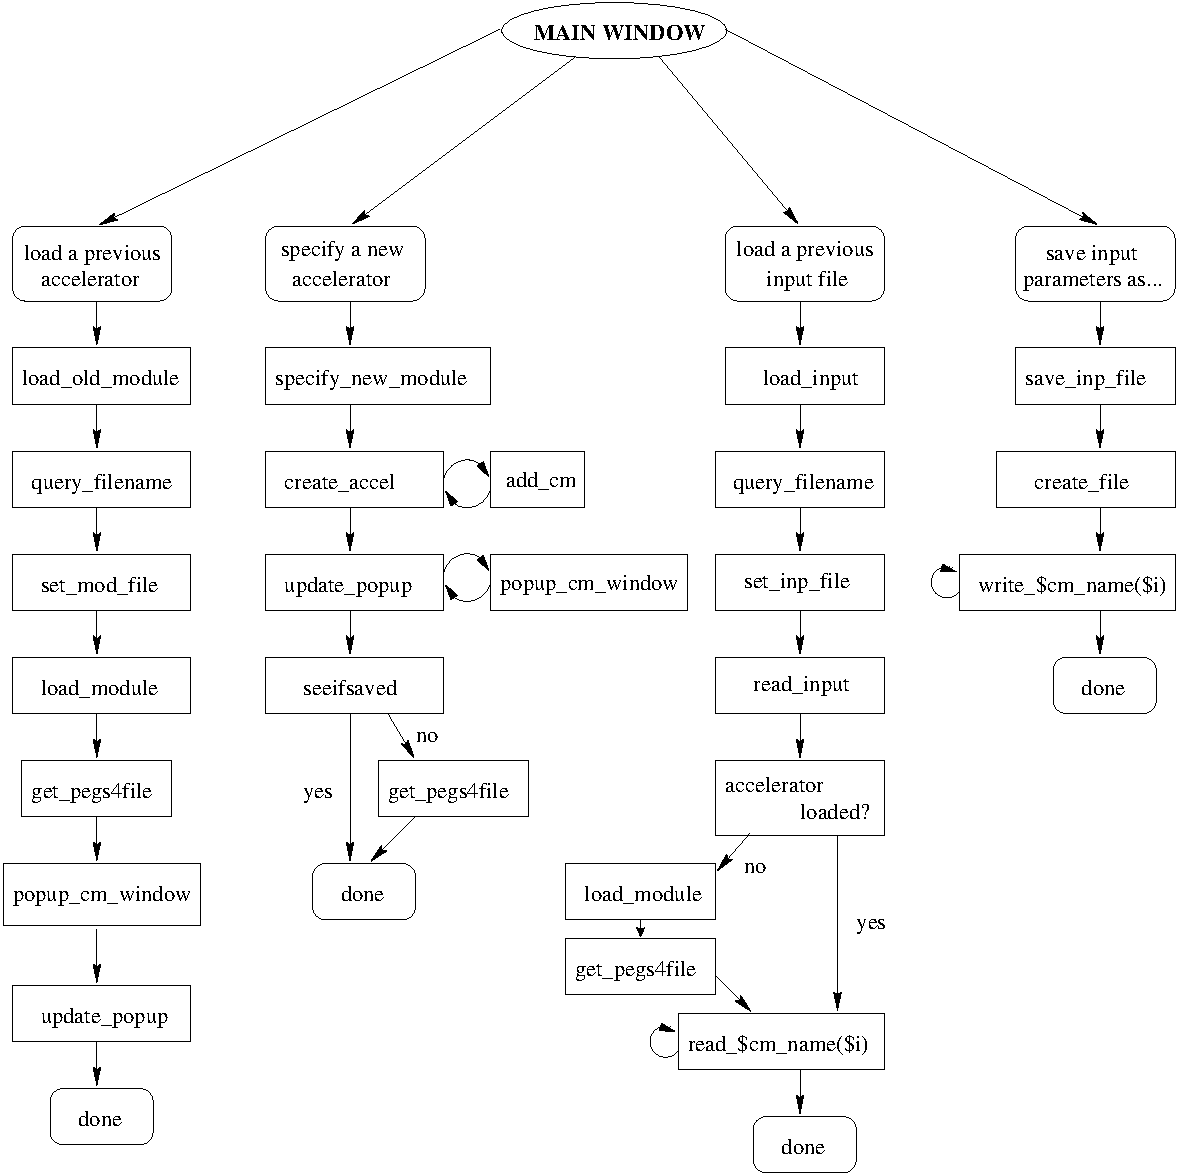
\includegraphics[width=\textwidth]{figures/main_flow_portrait}
\caption{Flow diagram of the procedure accessible from the top window of
the GUI.  Procedure names are in rectangular boxes.  Not all procedures
are shown;  ``done'' represents the point at which procedures involved in
setting parameters are used.\label{flowfig}}
\end{figure}


\section{Adding a Component Module to the Package}
Let the new CM be called ``NEWCM''.  Since there are 16 now we'll say
it's the 17$^{th}$ CM.
\begin{enumerate}
\item In {\tt beam\_params.tcl}, add ``NEWCM'' to the end of the array
{\tt cm\_names} with {\tt set cm\_names(17) ``NEWCM''}.

\item Since there are now 17 CMs, in {\tt create\_accel.tcl} you will have to
change 16 to 17 in the {\sf create\_accel} procedure:
\begin{verbatim}
    # add listbox, scrollbar, insert all availabel CM names
    listbox $top.l.list -height 10 -yscrollcommand "$top.l.scrl set" \
       -bg white
    for {set i 1} {$i <= 16} {incr i} {
       $top.l.list insert end $cm_names($i)
    }
    scrollbar $top.l.scrl -command "$top.l.list yview"
    pack $top.l.scrl -side right -fill y
    pack $top.l.list -side left -fill x -fill y
\end{verbatim}
and in the {\sf add\_cm} procedure:
\begin{verbatim}
    for {set i 1} {$i<=16} {incr i} {
       if [string compare $new_cm_name $cm_names($i)]==0 {
          set index [incr i -1]
          break
       }
    }
\end{verbatim}
\item In {\sf load\_module.tcl}, change 16 to 17 in
\begin{verbatim}
        for {set j 1} {$j <= 16} {incr j} {
            # look for a match in cm_names to get cm_type
            if [string compare $cm_names($j) $str]==0 {
                set found 1
                incr num_cm
                incr i
                set cm_type($i) $j
            }
        }
\end{verbatim}
\item In {\tt draw\_accel.tcl}, you will have to make an addition to the
{\sf get\_zmax} procedure in order to determine the where the CM ends.
What that value will be depends entirely upon the input parameters for it.

\item The biggest part of adding a new CM is making the code for it,
\ie~newcm.tcl.  To accomplish this, it is easiest to copy the code for the
CM which most closely resembles it in input format to the new file and
begin editing from that starting point.
\end{enumerate}

\section{Naming Conventions}

The variable naming conventions are given in this section.  They are
tabulated with the variable name used in the BEAM code.  The main
parameters are those defined in the procedure {\sf set\_main\_parameters}.
For those parameters which have multiple options instead of numerical
values, an option menu is created.  The options available to a
parameter I are defined in {\tt beam\_params.tcl} as {\tt options(I,J)},
where J is an integer.

If a variable is presented in the tables as having forward slashes in
its index, there are multiple variables, \ie~\verb+s9vals(1/2/3,i)+
means there are \verb+s9vals(1,i)+, \verb+s9vals(2,i)+,
and \verb+s9vals(3,i)+ variables.

For the CMs, the variable naming follows quite closely to the way they
are presented in the user manual.  {\tt cm\_type} is an array which holds an
integer corresponding to one of the available CMs for each of the CMs
used.  {\tt cm\_ident} is an array which holds identification strings for each
of the CMs used.  {\tt cm\_names} is an array containing strings ``SLABS'',
``APPLICAT'', {\it etc.}, in the order they are presented in the manual,
for use with {\tt cm\_type}.  Then for the \$id$^{\rm th}$ CM in the
accelerator, {\tt cm\_type(\$id)}
is a number corresponding to what type of CM \$id is in {\tt cm\_names} and
{\tt cm\_ident(\$id)} is its identifying string.  So if CM \#2 is a SLABS CM,
to get the string ``SLABS'', you would use {\tt \$cm\_names(\$cm\_type(2))}.


\subsection{GUI variables}

\begin{tabular}{|p{4.5cm}|p{11.5cm}|}\hline
rootx & the x-coordinate of the upper left corner of the first window \\
rooty & the y-coordinate of the upper left corner of the first window \\
helvfont & helvetica font \\
start\_dir & the directory the GUI was started in \\
inp\_file & the full input filename (including directory tree)\\
inp\_base & the base name of the input file (no tree, no extension) \\
inp\_file\_dir & the directory of the input file \\
mod\_file & the full name of the module file \\
mod\_base & the base name of the module file \\
pegs4filename & the full name of the PEGS4 data file (including tree) \\
colorlist & a list of colors to be associated with meida in drawing \\
medium(i), i=1,nmed & media available from PEGS4 file \\
nmed & the number of media read in from the PEGS4 file \\
num\_cm & the number of CMs used \\
cm\_names & an array of CM names \\
cm\_ident & an array to hold the identifying strings for each CM \\
cm\_type & an array to hold numbers which correspond to what type of CM
it is \\ \hline
\end{tabular}

\subsection{Main parameters}

\begin{tabular}{|p{4.5cm}|p{11.5cm}|}\hline
values(1) & TITLE \\
values(2) & MEDIUM for nominal air \\
values(3) & IWATCH \\
values(4) & ISTORE \\
values(5) & IRESUME\\
values(6) & IO\_OPT\\
values(7) & IDAT\\
values(8) & LATCH\_OPTION\\
values(9) & IZLAST\\
values(10) & NCASE\\
values(11) & IXX\\
values(12) & JXX\\
values(13) & TIMMAX\\
values(14) & IBRSPL, Brem splitting (none, uniform, selective)\\
values(15) & NBRSPL\\
sbrem(1/2/3) & FS, SSD, NMIN\\
values(16) & IRRLTT\\
values(17) & IQIN, Incident particle\\
values(18) & ISOURC, Source number\\
srcopts(1/2/3/4) & Four source options maximum for any source\\
s1opt & source 1 option, circular or square \\
s3opt & source 3 option, vertical or horizontal \\
s9vals(1/2/3,i) & Source 9 options \\
spcnam15 & Filename for source 15\\
spcnam21 & Filename for source 21\\
spcnam31 & Filename for source 31\\
monoen  & Monoenergetic or spectrum source \\
Ein\_val & Kinetic energy of source, EIN\\
spec\_file & Spectrum filename, FILNAM \\
ioutsp & IOUTSP \\
values(19) & ESTEPE\\
values(20) & SMAX\\
values(21) & ECUTIN\\
values(22) & PCUTIN\\
vaules(23) & IDORAY\\
values(24) & IREJCT\_GLOBAL\\
values(25) & ESAVE\_GLOBAL\\
values(26) & IFLUOR\\
ifluor\_opts(1,i) & effective Z, IZ\\
ifluor\_opts(2,i) & from region, IREGLO\\
ifluor\_opts(3,i) & to region, IREGHI\\
values(27) & IFORCE\\
force\_bdd(1/2/3/4) & NFMIN,NFMAX,NFCMIN,NFCMAX\\
\hline\end{tabular}

\noindent
\begin{tabular}{|p{4.5cm}|p{11.5cm}|}\hline
values(28) & NSC\_PLANES\\
values(28,1,i) & CM number for plane iscore, IPLANE\_to\_CM(I) \\
values(28,2,iscore) & NSC\_ZONES(ISCORE)\\
values(28,3,iscore) & MZONE\_TYPE(ISCORE)\\
values(28,4,iscore,i) & (RSCORE\_ZONE(ISCORE,I), I=1,NSC\_ZONES)\\
values(29) & ITDOSE\_ON \\
values(29,1/2) &      ICM\_CONTAM, IQ\_CONTAM \\
values(29,3) & LNEXC \\
l\_n\_exc & L\_N\_EXC(I,J), J=1, 31\\
exc & Used to hold an on/off array for exclusive filters \\
values(29,4) & LNINC \\
l\_n\_inc & L\_N\_INC(I,J), J=1, 31\\
inc & Used to hold an on/off array for inclusive filters \\
values(30) & Z\_min\_CM(1) \\
values(40) & ICM\_SPLIT \\ \hline
\end{tabular}

\subsection{APPLICAT}

\begin{tabular}{|p{4.5cm}|p{11.5cm}|}\hline
cmval(id,0) & RMAX\_CM(ICM)\\
cmval(id,1) & TITLE \\
cmval(id,2) & ZBACK \\
cmval(id,3,0/1) & N, ISHAPE \\
cmval(id,4,0/1/$\ldots$/7,I) & ZMIN(I), ZTHICK(I), XMIN(I),
       YMIN(I), WIDTHX(I), WIDTHY(I), DOSE\_ZONE, IREGION\_TO\_BIT  \\
cmval(id,6,0/1/2/3) & ECUT, PCUT, DOSE\_ZONE\_AIR, IREGION\_TO\_BIT\_AIR \\
cmval(id,7,I) & MED\_IN \\ \hline
\end{tabular}

\subsection{BLOCK}

\begin{tabular}{|p{4.5cm}|p{11.5cm}|}\hline
cmval(id,0) &  RMAX\_CM(ICM)\\
cmval(id,1) &  TITLE \\
cmval(id,2,0/1/2) &  ZMIN, ZMAX, ZFOCUS\\
cmval(id,3) &  ISUB\_MAX \\
cmval(id,4,j) &  NSUB(J)\\
cmval(id,4,j,0/1,i) &  XHI\_POINT(I,J),YHI\_POINT(I,J)\\
cmval(id,5,0/1/2/3) & XPMAX,YPMAX,XNMAX,YNMAX\\
cmval(id,6,0/1/2/3) &   ECUT, PCUT, DOSE\_ZONE, IREGION\_TO\_BIT \\
cmval(id,7,0/1/2/3) &   ECUT, PCUT, DOSE\_ZONE, IREGION\_TO\_BIT \\
cmval(id,8) & MED\_IN \\
cmval(id,9,0/1/2/3) & ECUT, PCUT, DOSE\_ZONE, IREGION\_TO\_BIT \\
cmval(id,10) & MED\_IN \\ \hline
\end{tabular}

\subsection{CHAMBER}

\begin{tabular}{|p{4.5cm}|p{11.5cm}|}\hline
cmval(id,0) & RMAX\_CM(ICM)\\
cmval(id,1)   & TITLE\\
cmval(id,2)    &ZMIN    \\
cmval(id,3,0/1/2)    &N\_TOP, N\_CHM, N\_BOT \\
top\_identical & flag: 1 if top layers identical, 0 if not\\
chm\_identical & flag: 1 if chamber layers identical, 0 if defined
individually, 2 if defined in groups\\
bot\_identical & flag: 1 if bottom layers identical, 0 if not\\
\hline Top part     & \\ \hline
cmval(id,4,0,0/1/2,i)   &each layer, ZTHICK, RCYS , NFLAG \\
cmval(id,4,1,0/1/2/3,i)   & each layer, inner cylinders,
ECUT, PCUT, DOSE\_ZONE, IREGION\_TO\_BIT\\
cmval(id,4,2,i)   &each layer, inner cylinders, MED\_IN\\
cmval(id,4,3,0/1/2/3,i)   &
each layer, outer annuli, ECUT, PCUT, DOSE\_ZONE, IREGION\_TO\_BIT\\
cmval(id,4,4,i)   &each layer, outer annuli, MED\_IN\\
\hline Chamber/phantom part  & \\ \hline
cmval(id,5,0,0/1/2) &  RCYS(1,1), RCYS(1,2), RCYS(1,3)\\
cmval(id,5,1,0/1,i)   &each layer, ZTHICK, NFLAG\\
cmval(id,5,2,0/1/2/3,i) &
each layer, ECUT, PCUT, DOSE\_ZONE, IREGION\_TO\_BIT\\
cmval(id,5,3,i)   &each layer, MED\_IN \\
cmval(id,5,4,0/1/2/3)   &
chamber wall, ECUT, PCUT, DOSE\_ZONE, IREGION\_TO\_BIT\\
cmval(id,5,5)   &chamber wall, MED\_IN  \\
cmval(id,5,6,0/1/2/3)   & gap, ECUT, PCUT, DOSE\_ZONE, IREGION\_TO\_BIT\\
cmval(id,5,7)   &gap, MED\_IN  \\
cmval(id,5,8,0/1/2/3)   &
container wall, ECUT, PCUT, DOSE\_ZONE, IREGION\_TO\_BIT\\
cmval(id,5,9)   &container wall, MED\_IN\\
\hline Bottom part   & \\ \hline
cmval(id,6,0,0/1/2,i)   &each layer, ZTHICK, RCYS , NFLAG\\
cmval(id,6,1,0/1/2/3,i)   &
each layer, inner cylinders, ECUT, PCUT, DOSE\_ZONE, IREGION\_TO\_BIT\\
cmval(id,6,2,i)   &each layer, inner cylinders, MED\_IN\\
cmval(id,6,3,0/1/2/3,i)   &each layer, outer annuli,
ECUT, PCUT, DOSE\_ZONE, IREGION\_TO\_BIT\\
cmval(id,6,4,i)   &each layer, outer annuli, MED\_IN\\
cmval(id,7)   & MRNGE \\\hline
\end{tabular}

\subsection{CIRCAPP}

\begin{tabular}{|p{4.5cm}|p{11.5cm}|}\hline
cmval(id,0) &  RMAX\_CM(ICM)\\
cmval(id,1) &  TITLE \\
cmval(id,2) &  ZBACK\\
cmval(id,3) &  N, number of layers\\
cmval(id,4,0/1/$\ldots$/6,i) & ZMIN(I), ZTHICK(I), ROPEN(I), XOUTER(I),
YOUTER(I), DOSE\_ZONE(I), IREGION\_TO\_BIT(I)\\
cmval(id,5,0/1/2/3) & ECUT, PCUT, DOSE\_ZONE\_AIR, IREGION\_TO\_BIT\_AIR\\
cmval(id,6,i) & MED\_IN \\ \hline
\end{tabular}

\subsection{CONESTAK}

\begin{tabular}{|p{4.5cm}|p{11.5cm}|}\hline
cmval(id,0) &  RMAX\_CM(ICM) \\
cmval(id,1) & TITLE \\
cmval(id,2,0/1) &  ZMIN, RBN \\
owall\_conestak(id) & 0 for no wall, 1 for a wall \\
cmval(id,3) &  ISCM\_MAX, Number of conical layers \\
cmval(id,4,0/1/2,i) & each layer, ZTHICK(I), RMIN(I), RMAX(I)\\
cmval(id,5,0/1/2/3) & outer wall, ECUT, PCUT, DOSE\_ZONE, IREGION\_TO\_BIT \\
cmval(id,6) & outer wall,  MED\_IN \\
cmval(id,7,i,0/1/2/3) & each layer inside cone, ECUT, PCUT, DOSE\_ZONE, IREGION\_TO\_BIT \\
cmval(id,8,i) & each layer inside cone, MED\_IN \\
cmval(id,9,i,0/1/2/3) & each layer outside cone, ECUT, PCUT, DOSE\_ZONE, IREGION\_TO\_BIT \\
cmval(id,10,i) & each layer, outside cone, MED\_IN \\\hline
\end{tabular}

\subsection{CONS3R}

\begin{tabular}{|p{4.5cm}|p{11.5cm}|}\hline
cmval(id,0) &  RMAX\_CM(ICM)\\
cmval(id,1) &  TITLE \\
cmval(id,2) &  ZMIN \\
cmval(id,3) &  ZTHICK \\
cmval(id,4) &  NUM\_NODE \\
cmval(id,5,0/1,i) &  ZCORNER(I), RCORNER(I) \\
cmval(id,6,0,0/1/2/3/4/5) & inner ECUT, PCUT, DOSE\_ZONE, IREGION\_TO\_BIT,
IREJCTIN, MED\_IN \\
cmval(id,6,1,0/1/2/3/4/5) & outer ECUT, PCUT, DOSE\_ZONE, IREGION\_TO\_BIT,
IREJCTIN, MED\_IN \\\hline
\end{tabular}

\subsection{FLATFILT}

\begin{tabular}{|p{4.5cm}|p{11.5cm}|}\hline
cmval(id,0) &  RMAX\_CM(ICM) \\
cmval(id,1) &  TITLE (60A1) \\
cmval(id,2) &  ZMIN \\
cmval(id,3) &  ISCM\_NO (number of layers)\\
cmval(id,4,0/1,i) & each layer,  ISSCM\_NO(I), ZTHICK(I)\\
cmval(id,5,i,j) & each layer, cone,  RTOP(I,J) \\
cmval(id,6,i,j) & each layer, cone,  RBOT(I,J) \\
cmval(id,7,0/1/2/3,i,j) & each layer, cone,  ECUT, PCUT, DOSE\_ZONE, IREGION\_TO\_BIT \\
cmval(id,8,j) & each cone,  MED\_IN \\\hline
\end{tabular}

\subsection{JAWS}

\begin{tabular}{|p{4.5cm}|p{11.5cm}|}\hline
cmval(id,0) &  RMAX\_CM(ICM\_JAWS) \\
cmval(id,1) &  TITLE \\
cmval(id,2) &  ISCM\_MAX, Number of paired bars or jaws\\
cmval(id,3,i) & each pair, XY\_CHOICE \\
cmval(id,4,0/1/2/3/4/5,i) & each pair, ZMIN(I), ZMAX(I), XFP(I), XBP(I), XFN(I), XBN(I) \\
cmval(id,5,0/1/2/3) & interior, ECUT, PCUT, DOSE\_ZONE, IREGION\_to\_BIT \\
cmval(id,6,0/1/2/3,i) & each pair, ECUT, PCUT, DOSE\_ZONE, IREGION\_TO\_BIT \\
cmval(id,7,i) & each pair, MED\_IN \\\hline
\end{tabular}

\subsection{PYRAMIDS}

\begin{tabular}{|p{4.5cm}|p{11.5cm}|}\hline
cmval(id,0) &  RMAX\_CM(ICM)\\
cmval(id,1) &  TITLE \\
cmval(id,2,0/1) &  ISCM\_MAX, IFILL \\
cmval(id,3,0/1/$\ldots$/11) &  ZMIN(I), ZMAX(I), XFP(I),
       XBP(I), XFN(I), XBN(I), YFP(I), YBP(I), YFN(I),
       YBN(I),XMAX(I), YMAX(I) \\
cmval(id,4,0/1/2/3) & air, ECUT, PCUT, DOSE\_ZONE, IREGION\_TO\_BIT \\
cmval(id,5,0/1/2/3,i) & each layer, opening, ECUT, PCUT, DOSE\_ZONE, IREGION\_TO\_BIT\\
cmval(id,6,i) & each layer, opening, MED\_IN \\
cmval(id,7,0/1/2/3,i) & each layer, surrounding, ECUT, PCUT, DOSE\_ZONE, IREGION\_TO\_BIT \\
cmval(id,8,i) &  each layer, surrounding, MED\_IN \\\hline
 \end{tabular}

\subsection{SIDETUBE}

\begin{tabular}{|p{4.5cm}|p{11.5cm}|}\hline
cmval(id,0) &  RMAX\_CM(ICM) \\
cmval(id,1) &  TITLE \\
cmval(id,2) &  ZMIN \\
cmval(id,3) &  ZTHICK \\
cmval(id,4) &  ZCYL \\
cmval(id,5,0/1) &  XMIN, XMAX \\
cmval(id,6) &  N, Number of coaxial cylinders. \\
cmval(id,7,i) &  each cylinder, R(I) \\
cmval(id,8,0/1/2/3,i) &  each cylinder, ECUT, PCUT, DOSE\_ZONE, IREGION\_TO\_BIT\\
cmval(id,9,i) &  each cylinder, MED\_IN \\\hline
\end{tabular}

\subsection{MESH}

\begin{tabular}{|p{4.5cm}|p{11.5cm}|}\hline
cmval(id,0) &  RMAX\_CM \\
cmval(id,1) &  TITLE \\
cmval(id,2) &  ZMIN \\
cmval(id,3,0/1/2/3) &  X\_AIR\_WIDTH, Y\_AIR\_WIDTH, WIRE\_WIDTH, WIRE\_THICK \\
cmval(id,4,0/1) & XTOTAL, YTOTAL \\
cmval(id,5,0/1/2/3) & inside, ECUT,PCUT,DOSE\_ZONE,IR\_TO\_BIT\\
cmval(id,6,0/1/2/3) & wire, ECUT,PCUT,DOSE\_ZONE,IR\_TO\_BIT \\
cmval(id,7) & wire, MED\_IN \\\hline
\end{tabular}

\subsubsection{Adjusting the mesh to fit the cells}
\begin{figure}[htbp]
\vspace{1.8in}
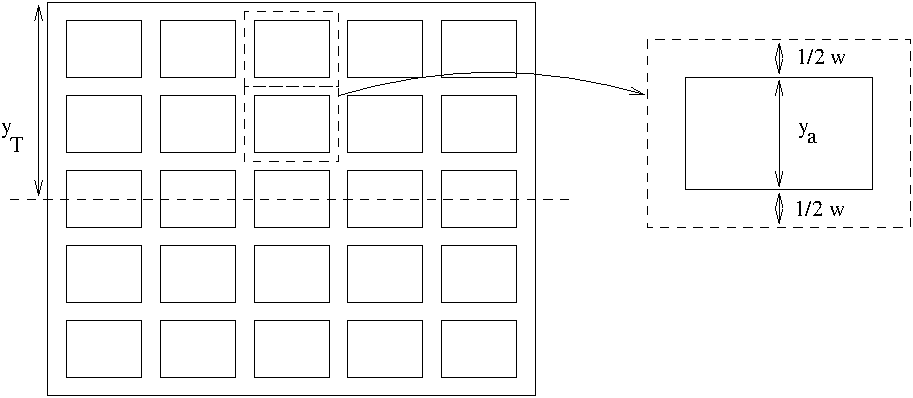
\includegraphics{figures/meshfig}
\caption{Diagram of a MESH.  \label{meshfig}}
\end{figure}

The user inputs the wire width, $w$, and the x and y air widths, $x_a$
and $y_a$.  From these the number of holes in x and y can be calculated.
The problem is that if the x or y total half-width ($x_T$, $y_T$)
isn't the proper size to accomodate an odd integer number of air holes it
has to be resized to do so.

Adding in the y-direction gives
$${\rm half-width = 1/2 hole + 1/2 wire + n (hole+wire) + 1/2 wire}$$
$$y_T=(n+\frac{1}{2})y_a+(n+1)w$$
$$2n=\frac{2y_T-y_a-2w}{y_a+w}$$
where n is the number of cells in half of the y-direction, not including
the central cell.  $2n$ is then the number of cells in the y-direction
not including the central cell.  This number must be forced to be an
even integer.

If it's not an integer, it is set to the next highest integer number.  If
this number is not even, it is reduced again to the next lowest
integer.  Then the total y-width of the mesh is reset to accomodate this
number of cells (+1, the central one) of the widths specified:
$$y_T=\frac{1}{2}y_a+w+n(y_a+w)$$

\subsection{MIRROR}

\begin{tabular}{|p{4.5cm}|p{11.5cm}|}\hline
cmval(id,0) &  RMAX\_CM(ICM) \\
cmval(id,1) &  TITLE \\
cmval(id,2,0/1) &  ZMIN, ZTHICK \\
cmval(id,3,0/1) &  XFMIN, XBMIN \\
cmval(id,4) &  N, Number of layers  \\
cmval(id,5,i) &  DTHICK(I) \\
cmval(id,6,0/1/2/3,i) & eack layer, ECUT, PCUT, DOSE\_ZONE, IREGION\_TO\_BIT \\
cmval(id,7,i) & each layer, MED\_IN \\
cmval(id,8,0/1/2/3) & behind mirror, ECUT, PCUT, DOSE\_ZONE, IREGION\_TO\_BIT\\
cmval(id,9) & behind mirror, MED\_IN \\
cmval(id,10,0/1/2/3) & front of mirror, ECUT, PCUT, DOSE\_ZONE, IREGION\_TO\_BIT\\
cmval(id,11) & front of mirror, MED\_IN \\\hline
\end{tabular}

\subsubsection{Finding the angle between the z-axis and the mirror}
\begin{figure}[htbp]
\vspace{1.8in}
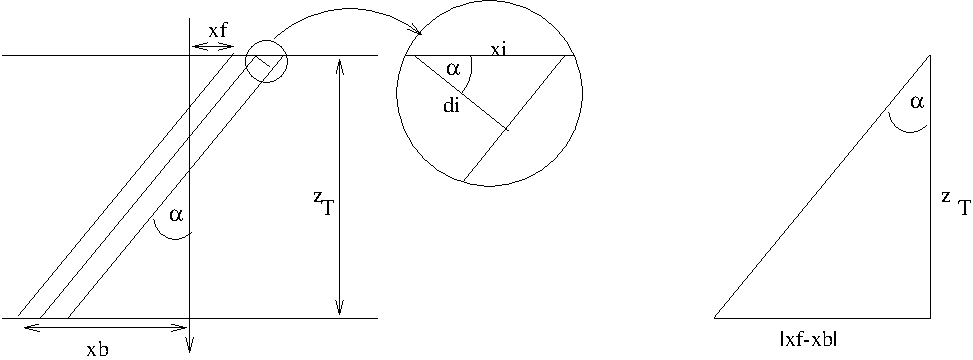
\includegraphics{figures/mirrorfig}
\caption{Diagram of a mirror.  $d_i$, $x_b$, $x_f$ and $z_T$ are user-defined.
\label{mirrorfig}}
\end{figure}

In the inputs, $d_i$ is the thickness of layer $i$.  To draw the mirror
we need to find the x-width of the layer.  This is given by
$$ \cos\alpha=\frac{d_i}{x_i}$$
or
$$ x_i=\frac{d_i}{\cos\alpha}$$
Where the angle $\alpha$ is as shown in figure \ref{mirrorfig}, the
angle between the z-axis and the parallel lines of the layers in the mirror.

The angle $\alpha$ is as shown in the right triangle in figure \ref{mirrorfig},
$$\tan\alpha=\frac{|x_f-x_b|}{z_T}$$
$$\alpha=\tan^{-1}\left(\frac{|x_f-x_b|}{z_T}\right)$$

\subsection{MLC}

\begin{tabular}{|p{4.5cm}|p{11.5cm}|}\hline
cmval(id,0) &  RMAX\_CM(ICM) \\
cmval(id,1) &  TITLE \\
cmval(id,2) &  IDMLFC \\
cmval(id,3) &  ZMIN \\
cmval(id,4) &  ZTHICK \\
cmval(id,5) &  NUM\_LEAF, TWIDTH \\
cmval(id,6) &  ZFOCUS(1) \\
cmval(id,7) &  ZFOCUS(2) \\
cmval(id,8,0/1/2,i) &  NEG, POS, NUM for group i\\
cmval(id,9,0/1/2/3) &  inside, ECUT, PCUT, DOSE\_ZONE, IREGION\_TO\_BIT\\
cmval(id,10) &  inside, MED\_IN \\
cmval(id,11,0/1/2/3) &  leaves, ECUT, PCUT, DOSE\_ZONE, IREGION\_TO\_BIT\\
cmval(id,12) &  leaves, MED\_IN \\
ngroups & number of groups \\ \hline
\end{tabular}

\subsubsection{Finding the x-coordinate at the bottom}
\begin{figure}[htbp]
\vspace{1.8in}
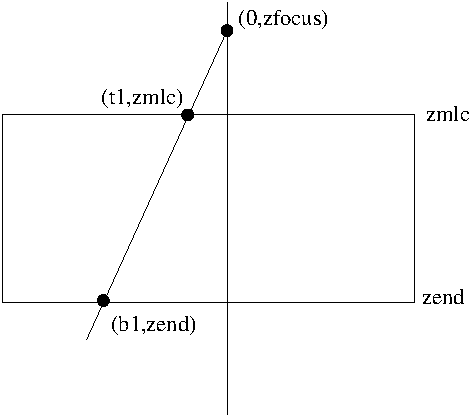
\includegraphics{figures/mlcfig}
\caption{Diagram of a MLC.  \label{mlcfig}}
\end{figure}

This CM has a focal point for the sides and for the ends of the
collimator leaves.  The user defines the coordinates at the top of the
CM, so to draw the sides and ends the coordinates at the bottom of the
CM must be calculated.  Simply draw a line from the focal point on the
z-axis (0,$zfocus$) through the point at the top ($t_1$,$zmlc$) to get the
equation in x and z
$$z=mx+b$$
$$zfocus=b$$
$$zmlc=mt_1+zfocus \rightarrow m=\frac{zmlc-zfocus}{t_1}$$
We want to get the point at the bottom, ($b_1$,$zend$)
$$zend=\frac{zmlc-zfocus}{t_1}b_1+zfocus$$
or
$$b_1=t_1\frac{zend-zfocus}{zmlc-zfocus}$$

\subsection{XTUBE}

\begin{tabular}{|p{4.5cm}|p{11.5cm}|}\hline
cmval(id,0) &  RMAX\_CM(ICM) \\
cmval(id,1) &  TITLE \\
cmval(id,2,0/1) &  ZMIN, ZTHICK \\
cmval(id,3) &  ANGLEI \\
cmval(id,4) &  N, Number of layers in the target \\
cmval(id,5,i) &  each layer, DTHICK(I) \\
cmval(id,6,0/1/2/3,i) &  each layer, ECUT, PCUT, DOSE\_ZONE, IREGION\_TO\_BIT\\
cmval(id,7,i) &  each layer, MED\_IN \\
cmval(id,8,0/1/2/3) &  front of target, ECUT, PCUT, DOSE\_ZONE, IREGION\_TO\_BIT\\
cmval(id,9,0/1/2/3) &  target holder, ECUT, PCUT, DOSE\_ZONE, IREGION\_TO\_BIT\\
cmval(id,10) & target holder, MED\_IN \\\hline
\end{tabular}

\subsubsection{Finding the x-coordinate given the thickness of the layer}
\begin{figure}[htbp]
\vspace{1.6in}
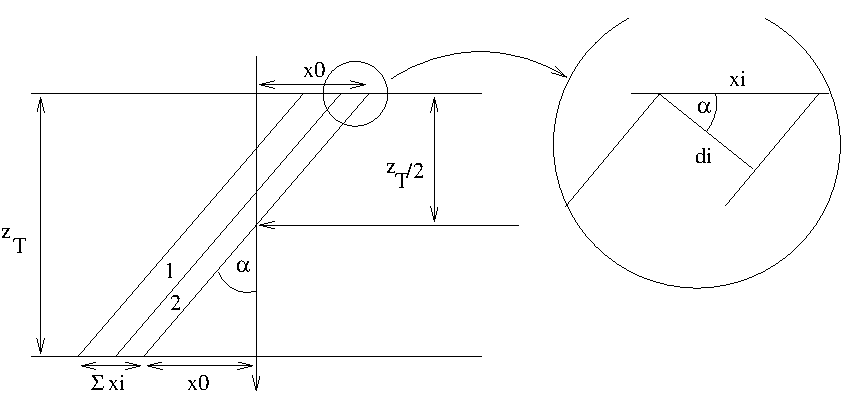
\includegraphics{figures/xtubefig}
\caption{Diagram of an xtube.  \label{xtubefig}}
\end{figure}
The thickness of each layer is defined in the inputs, but we need the
x-distance between layers in order to draw them.  From the diagram,
$\cos\alpha=d_i/x_i$, where $d_i$ is the user-input thickness of the
layer and $\alpha$ is the user-input angle between the target and
z-axis.  To draw the first layer, \eg, we need the four points xtop1,
xbot1, xtop2 and xbot2.  The total x-width at the top and bottom of all
layers is
$$\sum_i x_i=\sum_i \frac{d_i}{\cos\alpha} $$
The top and bottom x-distances of the last layer are given by
$x_0=\frac{z_T}{2}\tan\alpha$.
Then we have
\begin{eqnarray}
 xtop1&=&x_0-\sum_i x_i\nonumber\\
 xtop2&=&x_0+x_1-\sum_i x_i \nonumber\\
 xbot1&=&-x_0-\sum_i x_i \nonumber\\
 xbot2&=&-x_0+x_1-\sum_i x_i \nonumber\\ \nonumber
\end{eqnarray}
\noindent defining the polygons of the xtube layers.

\subsection{SLABS}

\begin{tabular}{|p{4.5cm}|p{11.5cm}|}\hline
cmval(id,0) &  RMAX\_CM(ICM)\\
cmval(id,1) &  TITLE \\
cmval(id,2) &  N,  Number of planar slabs\\
cmval(id,3) &  ZMIN \\
cmval(id,4,0/1/$\ldots$/6,i) & each layer, ZTHICK, ECUT, PCUT, DOSE\_ZONE,
IREGION\_TO\_BIT, ESAVEIN, MED\_IN    \\\hline
\end{tabular}

\subsection{ARCCHM}

\begin{tabular}{|p{4.5cm}|p{11.5cm}|}\hline
cmval(id,0) &  RMAX\_CM(ICM) \\
cmval(id,1) &  TITLE \\
cmval(id,2) &  ZSRC \\
cmval(id,3) &  ZRAD1 \\
cmval(id,4) &  NUMCHM \\
cmval(id,5) &  WIDTHCHM \\
cmval(id,6) &  WIDTHSEP \\
cmval(id,7) &  ARCTHICK \\
cmval(id,8) &  FRONTHCK \\
cmval(id,9) &  BACKTHCK \\
cmval(id,10) &  WIDXWALL \\
cmval(id,11,0/1) &  XMIN1, XMAX2 \\
cmval(id,12) &  ZMAX \\
cmval(id,13,j,0/1/2/3) &  each layer j (see manual), ECUT, PCUT, DOSE\_ZONE, IREGION\_TO\_BIT\\
cmval(id,14,j) &  each layer j, MED\_IN \\ \hline
\end{tabular}


\chapter{DOSXYZ GUI}

{\sffamily
\section{Introduction}
}

Currently the working source code for the GUI is stored in
\verb+$OMEGA_HOME/progs/gui+.
It is written in Tcl/Tk.  On this system, the
versions available are Tk version 4.1 and Tcl version 7.5 with wish
version 4.1 or wishx.  Use wishx if you want compatibility with the
SGIs here since they use an older version of wish which doesn't run the
script properly.  The use of older versions of tcl and tk are good for
portability.

At this time, the GUI is not portable to Windows or Mac because when
directory trees are specified I did not always use the 'file join' command but
simply put in forward slashes, '/'.

\section{Tcl/Tk Files for the GUI}

The files required for the GUI are listed in this section.
Figure~\ref{flowfig} shows a flow representation of how the procedures
interact with one another.

\begin{enumerate}
\item xyz\_gui is the main script for the DOSXYZ GUI.  It pops up the
main window from which DOSXYZ input files may be loaded and/or edited
and/or saved.

\item xyz\_parameters.tcl is a file containing parameters used in the
GUI.  For each variable the help text is set and a default value is
assigned if required (\ie~for an option menu).  It is read only once
when the GUI is started.

\item browser.tcl contains code for a directory browser.  It is the same
as query\_filename.tcl, but it does not use a filter.
\begin{enumerate}
\item proc browse \{ next\_proc\_name dir \} is the browser code.
\item proc set\_spec\_file \{ \} sets spec\_file to what the user has
selected in the textbox of the browser.
\end{enumerate}

\item create\_file.tcl contains the code to write the inputs to a file.
\begin{enumerate}
\item proc create\_file \{ file \} writes the inputs to $<$file$>$.
\item proc error\_flag \{ text \} puts an error message on the screen if
one of the required inputs is missing.
\end{enumerate}

\item define\_phantom.tcl contains code to define the phantom, either
with CT data or voxel-by-voxel.  These procedures are called from the
``Define phantom'' button on the main input window.
\begin{enumerate}
\item proc define\_phantom \{ \} puts up the proper window for data
input, depending on which method was selected on the main inputs
window.  If it is voxel-by-voxel, it puts up a window with buttons for
defining materials, x/y/z-voxel geometry as individually or groups,
izscan, and the media of the voxels.  If it is CT data, it puts up a
window with entry boxes for the filename to use (from which it reads the
media used) and other variables.
\item proc define\_nmed \{ \} puts up a window for the definition of
media and estepe for each medium.
\item proc define\_voxels \{ dir \} pops up a window for the definition,
in groups or individually, of voxels in direction \$dir (x, y, or z).
\item proc voxel\_med \{ \} puts up the window to assign media to the
voxels, in groups (from x/y/z, to x/y/z)
\item proc add\_group \{ w \} adds a group of voxels to the voxel\_med window.
\item proc define\_izscan \{ \} puts up a window to set the output to a
z-scan per page or an x-scan per page for groups of voxels, as above.
\item proc add\_scan\_group \{ w \} adds a new group (empty entries) to
the izscan window.
\end{enumerate}

\item help.tcl contains 2 small procedures that act as stepping-stones
to the help\_dialog and help\_gif routines in misc.tcl.
\begin{enumerate}
\item proc help \{ i \} is for help that does not require a picture.
\item proc help\_srcopts \{ w iopt \} is for help that needs a gif file
(\ie~source help).
\end{enumerate}

\item load\_input2.tcl contains procedures for loading a previous input file.
\begin{enumerate}
\item proc load\_input \{ \} calls query\_filename to search for the
file to load.
\item proc set\_inp\_file \{ tree filen \} sets the variable inp\_file
to that selected, then calls read\_input.
\item proc read\_input \{ \} opens the file and reads in the input parameters.
\end{enumerate}

\item misc.tcl contains two help dialog box routines and tk\_dialog.
\begin{enumerate}
\item proc help\_dialog \{ w title text bitmap default args \} is for
help that does not require a picture.  A text box with a scrollbar
displays the text associated with the variable.
\item proc help\_gif \{ w text iconfile \} is for help that requires a
gif file (\ie~source help).  The picture appears to the left and the
text with scrollbar to the right.
\item proc tk\_dialog \{ w title text bitmap default args \} is included
here to change the font and the width of the message box from the
default (it overrides the builtin function).
\end{enumerate}

\item query\_filename.tcl contains the code for browsing the directory tree.
\begin{enumerate}
\item proc query\_filename \{ next\_proc\_name dir ext \} pops up a
window with next\_proc\_name as the next procedure, dir as the starting
point in the directory tree and ext as the filter.
\item proc call\_next\_proc \{ next\_proc\_name \} calls the next
procedure.
\item proc update\_phantfile \{ tree filename \} set the variable
PhantFileName when it is this variable being set.
\end{enumerate}

\item save\_input.tcl contians code for saving the input file.
\begin{enumerate}
\item proc save\_input \{ \} calls query\_filename to get the name of
the file to save it as.
\item proc DoesInpFileExist \{ tree filename \} checks whether this file
exists and if it does, prompts the user with ``Are you sure?''
(overwrite\_prompt).
\item proc save\_inp\_file \{ tree filen \} sets the inp\_file variable
to its new value then calls create\_file to write it.
\item proc overwrite\_prompt \{ tree filename \} puts up a dialog box if
the file selected already exists.
\end{enumerate}

\item set\_main\_inputs.tcl contains code for the main input window.
\begin{enumerate}
\item proc edit\_parameters \{ \} pops up the main window and places the
main input parameter text boxes or option menus on it, as well as the
radiobuttons for how to define the voxels and the button to do it, and
the option menu for sources, which pops up the source option window
automatically.
\item proc set\_value \{ io iopt w \} set the value of a variable with
an option menu.
\item proc set\_presta \{ \} pops up a window to set the PRESTA inputs
if the default is not used.
\end{enumerate}

\item set\_source.tcl contains code for setting the source options.
\begin{enumerate}
\item proc set\_src\_options \{ iopt \} pops up the main source input
window, depending on which source was chosen.
\item proc enable \{ flag \} enables or disables buttons/menus/textboxes
depending on which source is chosen.
\item proc set\_inc\_or\_exc \{ parent index \} pops up a window in
which the user chooses LATCH bits for inclusive and/or exclusive filters.
\item proc close\_latbit \{ index \} saves the LATCH bit settings
selected in the variable latbit when the previous window is closed.
\end{enumerate}

\end{enumerate}

\begin{figure}[hp]
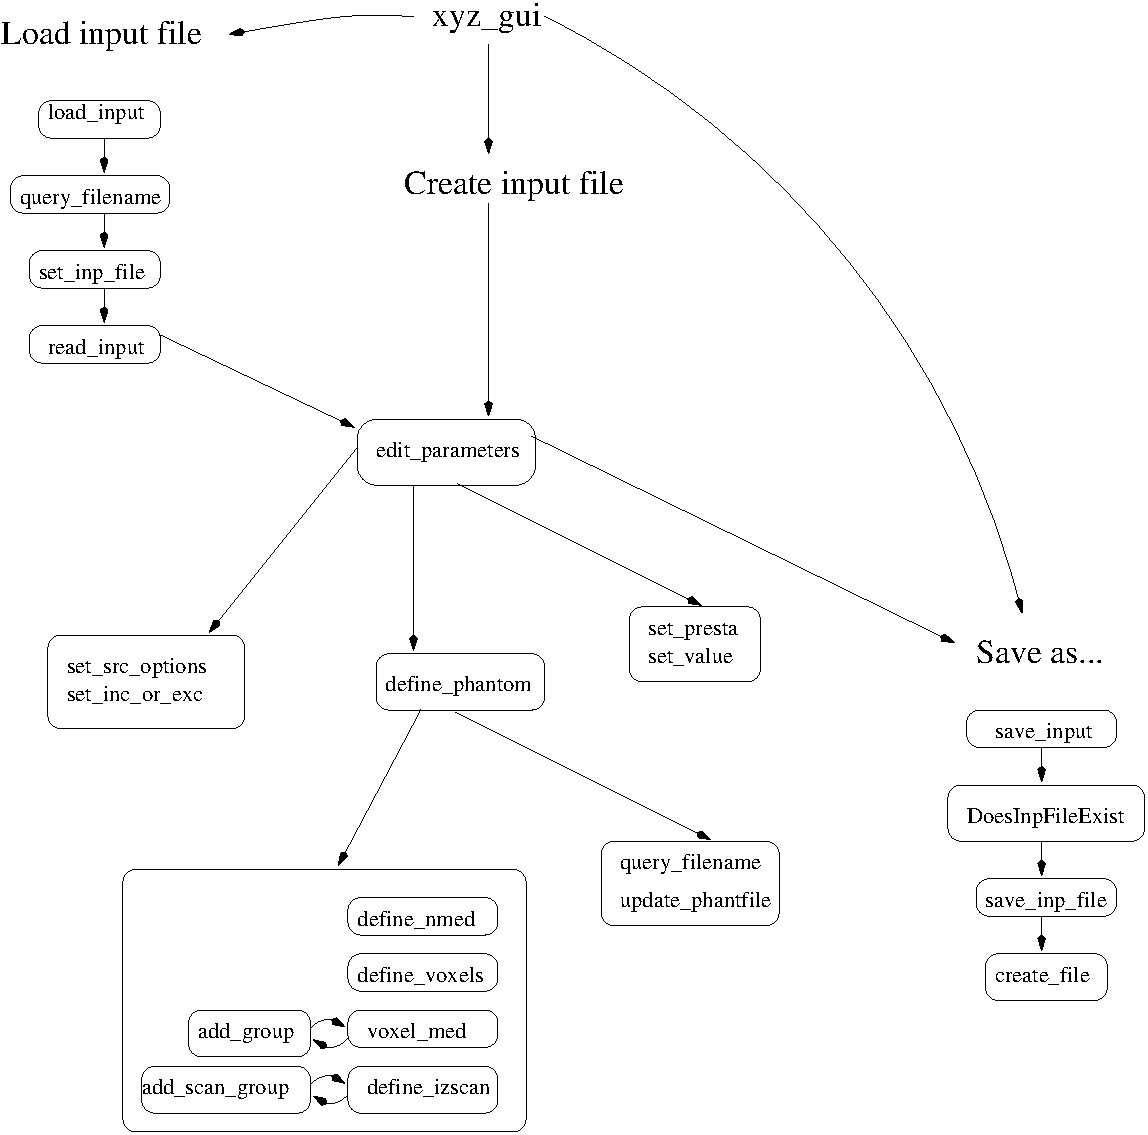
\includegraphics[width=16.5cm]{figures/flow_xyz}
\caption{A flow diagram of how the procedures interact.  Note that not
all are presented (those that are not directly linked to another).
\label{flowfig}}
\end{figure}

\section{Naming Conventions}

\subsection{Main}
\begin{tabular} {|p{1.5in}|p{3.75in}|}
\hline
Name & Meaning \\ \hline
values(1) & title \\
values(2) & nmed \\
CTdataflag & flag for ct/non-ct phantom\\
values(5) & ncase \\
values(6) & iwatch \\
values(7) & timmax \\
values(8) & inseed1 \\
values(9) & inseed2 \\
values(10) & beam\_size \\
values(11) & ismooth \\
values(12) & iresume \\
values(13) & idat \\
values(14) & ireject \\
values(15) & esave\_global \\
values(16) & presta inputs default/user set \\
values(16,0/1/2/3/4) & presta inputs \\
values(20) & zeroairdose \\
values(21) & doseprint \\
values(22) & max20 \\ \hline
\end{tabular}

\subsection{Source}

\begin{tabular} {|p{1.5in}|p{3.75in}|}
\hline
Name & Meaning \\ \hline
values(3) & electron, photon, positron option menu\\
values(4) & source number\\
numsrcopts(i) & for each source i, is the number of source options required.\\
srcoptnames(i,j) & for each source i, is the label used for source option j.\\
values(4,j) & value of source option j for the source selected.\\
Ein & energy of monoenergetic beam.\\
spec\_file & spectrum file for sources.\\
enflag & flag for the sources (ENFLAG)\\
medsur & medium surrounding phantom (MEDSUR) \\
dsurround & thickness of region surrounding phantom (DSURROUND).\\
values(17) & mode option menu (phase space file format) \\
values(18) & i\_bit\_filter \\
nbit1 &  number of bits to be used for the filter\\
nbit2 & number of bits to be used for the second half of the filter
(incluse and exclusive) (nbit1+nbit2 < 29) \\
inc & is an array of length 29 for inclulsive filter; if bit j is on,
inc(j)=1, else inc(j)=0\\
exc & is an array of length 29 for exclusive filter; if bit j is on,
exc(j)=1, else exc(j)=0\\
latbit(i) & holds the bits to include/exclude (i=1,nbit1 and i=nbit1+1,nbit2)\\
\hline
\end{tabular}

\subsection{Define media}

\begin{tabular} {|p{1.5in}|p{3.75in}|}
\hline
Name & Meaning \\ \hline
imax(0/1/2) & Number of voxels in X/Y/Z \\
medium(i) & Name of medium i  \\
ecutin &  electron cutoff energy\\
pcutin &  photon cutoff energy\\
estepm(i) & estepe for medium i \\
smax  & maximum step size, default 5cm \\
PhantFileName &  filename to be used for pahntom created by CT data.\\ \hline
\end{tabular}

\newpage
\subsection{Define voxel geometries}

\noindent If imax(0)$>$0, define individually.  Input x0,x1,x2,...,xN
(likewise for y and z):

\begin{tabular} {|p{1.5in}|p{3.75in}|}
\hline
Name & Meaning \\ \hline
ivox(0,i) & xi, x-coord of end of voxel (x(i-1) is the x-coord of start
of voxel) \\
ivox(1,i) & yi, y-coord of end of voxel (y(i-1) is the y-coord of start
of voxel) \\
ivox(2,i) & zi, z-coord of end of voxel (z(i-1) is the z-coord of start
of voxel) \\ \hline
\end{tabular}

\noindent If imax(0/1/2)$<$0, input min,width,number of voxels:

\begin{tabular} {|p{1.5in}|p{3.75in}|}
\hline
Name & Meaning \\ \hline
gvox(0,0) & min x for group i \\
gvox(0,i,1) & x-width for group i \\
gvox(0,i,2) & number of voxels with this width in group i \\
gvox(1,0) & min y for group i \\
gvox(1,i,1) & y-width for group i \\
gvox(1,i,2) & number of voxels with this width in group i \\
gvox(2,0) & min z for group i \\
gvox(2,i,1) & z-width for group i \\
gvox(2,i,2) & number of voxels with this width in group i \\ \hline
\end{tabular}

\subsection{Define voxel media}

\noindent Define material and density and IZSCAN in groups:

\begin{tabular} {|p{1.5in}|p{3.75in}|}
\hline
Name & Meaning \\ \hline
nrow & Number of material groups \\
izrow & Number of iz groups \\ \hline
\end{tabular}

\noindent For group i (i=1,nrow):

\begin{tabular} {|p{1.5in}|p{3.75in}|}
\hline
Name & Meaning \\ \hline
mvox(i,0,0) & x from    \\
mvox(i,0,1) & x to  \\
mvox(i,1,0) & y from  \\
mvox(i,1,1) & y to  \\
mvox(i,2,0) & z from  \\
mvox(i,2,1) & z to  \\
mvox(i,0) & material \\
mvox(i,1) & density \\ \hline
\end{tabular}

\noindent For group i (i=1,izrow):

\begin{tabular} {|p{1.5in}|p{3.75in}|}
\hline
Name & Meaning \\ \hline
izvox(i,0,0) & x from    \\
izvox(i,0,1) & x to  \\
izvox(i,1,0) & y from  \\
izvox(i,1,1) & y to  \\
izvox(i,2,0) & z from  \\
izvox(i,2,1) & z to  \\
izvox(i) & IZSCAN for group i \\ \hline
\end{tabular}



\end{document}
